\documentclass[a4paper]{article}

%\usepackage{a4wide,times}
\usepackage[english]{babel}
\usepackage[hidelinks]{hyperref}

% -----------------------------------------------
% especially use this for you code
% -----------------------------------------------

\usepackage{courier}
\usepackage{listings}
\usepackage{color}
\usepackage{graphicx}
\usepackage{amsmath}
\usepackage{amsfonts}
%\usepackage{math­de­sign}

\newcommand*\textcirc[1]{\textcircled{\raisebox{-0.6pt}{#1}}}



\definecolor{Gray}{gray}{0.95}


\usepackage{graphicx}
\usepackage[margin=1.5in]{geometry}
\renewcommand{\rmdefault}{pplx}



\usepackage{amssymb}
\newcommand{\idiv}{\mbox{\bf ~div~}} 
\newcommand{\imod}{\mbox{\bf ~mod~}} 
\newcommand{\band}{~\wedge~} 
\newcommand{\bor}{~\vee~} 
\newcommand{\true}{\mbox{\bf ~true~}} 
\newcommand{\false}{\mbox{\bf ~false~}} 
\newcommand{\IF}{\mbox{\bf if~}} 
\newcommand{\THEN}{\mbox{\bf ~then~}}
\newcommand{\ELSE}{\mbox{\bf else~}}
\newcommand{\END}{\mbox{\bf end}}
\newcommand{\WHILE}{\mbox{\bf while~}}
\newcommand{\DO}{\mbox{\bf ~do}}
\newcommand{\FOR}{\mbox{\bf for~}}
\newcommand{\TO}{\mbox{\bf ~to}}
\newcommand{\SKIP}{\mbox{\bf ~skip}}
\newcommand{\CONST}{\mbox{\bf const~}}
\newcommand{\ARRAY}{\mbox{\bf ~array~}}
\newcommand{\OF}{\mbox{\bf ~of~}}
\newcommand{\VAR}{\mbox{\bf var~}}
\newcommand{\vf}{\mbox{\sf vf}}
\newcommand{\ord}{\mbox{\sf ord}}
\newcommand{\imax}{\mbox{\bf ~max~}}
\newcommand{\imin}{\mbox{\bf ~min~}}
\newcommand{\Max}{\mbox{\sf Max}}
\newcommand{\Min}{\mbox{\sf Min}} 
\newcommand{\isqrt}{\mbox{\bf int\_sqrt}} 


% -- until here ---------------------------------

\begin{document}




\title{the Distributed Hash Tree
}
\date{\today}
\author{Wiebe-Marten Wijnja
}

\maketitle

\section{Abstract}

%Old abstract
Presented here is a novel data structure called the \textbf{Shuffled-Branch Treespace} that can be implemented on top of a distributed hash table. This data structure is then used as the building block of a \textbf{Distributed Hash Tree}, a new data structure that provides the possibility for users to secretly and securely collaborate on a fault-tolerant shared collection or tree of resources, without needing a central authority or a consensus-based system.


 Possible uses of Distributed Hash Trees include enabling the creation of a distributed version-control-system and distributed bulletin-boards.

%New abstract

\section{Introduction}

Two users, \textit{Alice} and \textit{Bob} want to secretly share information with each other remotely. They could send each other messages. However, this creates the need for them to know each other's identity and location. They do not want that. Also, as these messages can be followed by any person in-between them\footnote{In real life, this would be the messenger. In Computing Science, this might be a central server that both connect to, a `man in the middle' or  connected systems that pass on the message in a certain direction, such as those comprising the Internet Link Layer.}.\\

A different approach would be to store messages in a location that both could access, without third parties learning this location, or the location where the next message might appear. For a real-life analogy, one could picture them hiding the message in a hole in the desert at a certain latitude/longitude. In Computing Science, this could be done by storing message values in a \textbf{Distributed Hash Table} (Abbreviated as \textit{DHT}) at a \textit{key} known only to the users. But this only works for one message. They could create a whole list of locations for messages, but Alice and Bob might not have a secure channel to share this list of locations on, and the number of messages they want to send might increase beyond the length of locations they have. Also, when Alice and Bob try to save a message at the same time, the location is already filled on part of the DHT servers\footnote{Notice that we use the term \textit{server} in favor of `node' in the context of \textit{a machine that is part of the DHT network}. This is because the term \textit{node} is also used to describe \textit{an element of a tree}.}, creating an inconsistent state; and making it impossible for them to read the message from the other. A similar situation occurs when (because of technical failure) a message is dropped from the DHT before the other user could retrieve it.\\

Clearly, another solution is needed. To solve these problems, a system with the following features has to be created:

\begin{description}
	\item[Discovery] Users should be able to find out that new content has been added to the collection without needing an out-of-band notification.
	\item[Secrecy] DHT nodes and anyone else seeing the traffic should not be able to read the contents of stored values.
	\item[Immutability] Once a value is stored, it cannot be modified without invalidating it.
	\item[Exact Versioning] Content should be able to reference earlier content; the order of the elements should be absolute.
	\item[Fault Tolerance] When one value disappears from the DHT because of a technical failure, the rest of the system should be able to continue working, the rest of the content in the collection should still be accessible.
	\item[Authorization] Only persons that are allowed to should be able to append a collection.

\end{description}



Such a system could be used for a wide variety of applications that depend on (secret) collaboration of multiple parties on a collection of resources, without using a central authority. Some ideas could be:
\begin{itemize}
	\item A Distributed Bulletin-Board-like application similar to \textit{Reddit}, where users can read and write messages and reply to each other's messages.
	\item A Distributed Version Control System similar to \textit{Git}, where the system keeps track of a tree of edits in a file system.
\end{itemize}



\section{The Shuffled-Branch Tree}





\subsection{Iterative Hashing Dimensions}


\begin{description}
	

	\item[\textcircled{a}] Observe that when  $key_0 = hash(secret)$,a new key to store the next value can be inferred, by hashing the new $key$ again: $key_1 = hash(hash(secret)) = hash(key_0)$. This procedure can be repeated any $n \in \mathbb{N}$ number of times, providing locations to store any number of values: 
	
	$key_0 = hash(secret)$\\
	$key_1 = hash(hash(secret)) = hash(key_0)$\\
	$key_n = hash(key_{n-1})$
	
	The only information needed to move to the next index in this direction is the current hash.
	
	
	\item[\textcircled{b}] Instead, a secret value named the $salt$ can be concatenated\footnote{the concatenation operation is denoted as `$\parallel$'. Other operations such as $\oplus$ (exclusive or) might also be used for a similar effect, providing even more directions with the same level of secrecy.} to each current key before hashing it. This procedure can also be repeated any number of $n$ times: 
	
   	$key_0 = hash(secret \parallel salt)$ \\	
	$key_1 = hash(hash(secret \parallel salt) \parallel salt) = hash(key_0\parallel salt)$\\
	$key_n = hash(key_{n-1} \parallel salt)$	 
	
	To move to the next index in this direction, both the current hash as well as the salt have to be known.
	 
	\item[\textcircled{c}] It is also possible to use a $nonce$ at the innermost level, and instead of iteratively hashing, keep hashing the original secret, concatenated with the incremented nonce. This procedure can also be repeated any $n$ times:
	
	$key_0 = hash(secret \parallel 0)$ \\
	$key_1 = hash(secret \parallel 1)$ \\
	$key_n = hash(secret \parallel (n-1))$
	
	The only way to move to the next index in this direction, is to know the original secret, as well as the current value of the nonce.

\end{description}

This list is not exhaustive, but gives a good indication of key-transformations that can be applied using one-way hashing functions to move from one index to the next. \\


Notice that it is possible to combine above methods to create a key-space with multiple dimensions that can be used to store values in and read values from, as can be seen in more detail in Figure \ref{fig:combined_hashing_funcs}.  Notice that in the example posed in Figure \ref{fig:combined_hashing_funcs}, procedure \textcircled{b} could be applied to any other column besides column 0 as well, which would create a three-dimensional space. Then, procedure \textcircled{a} could again be applied to that, creating a four-dimensional space. This could be repeated ad-infinitum, although it has to be seen if there is a practical use for this. 


The difference in required information to move in a certain direction (or dimension) is an important property that will be used in the data structure we will describe shortly.


\begin{figure}

$$
\begin{bmatrix}
	key_{0,0} = hash(secret \parallel salt),      & key_{0,1} = hash(key_{0,0})  & \dots & key_{0,m} = hash(key_{0,m-1}) \\
	key_{1,0} = hash(key_{0,0} \parallel salt),   & key_{1,1} = hash(key_{1,0})  & \dots & key_{1,m} = hash(key_{0,m-1}) \\
	\vdots & \vdots & \ddots & \vdots \\
	key_{n,0} = hash(key_{n-1,0} \parallel salt), & key_{n,1} = hash(key_{n,0})  & \dots & key_{n,m} = hash(key_{n,m-1}) \\
\end{bmatrix}
$$

	\caption{
	\label{fig:combined_hashing_funcs}	
	A way to combine two iterative hashing procedures (in this case \textcircled{a} and \textcircled{b}) to create a two-dimensional key-space.
	}
\end{figure}

Also note that because one-way hashing functions (as the name implies) only move in \textit{one way}, even when given enough information to construct the next key from the current, it is still impossible to travel backwards (to the previous key). This means that it is also possible to share only \textit{part} of the keyspace with another user.\\


\subsection{Handling Latency, Concurrency-Problems and Faults}

This seems to work well: Given two users, \textit{Alice} and \textit{Bob}, that can only communicate through the DHT, \textit{Alice} can upload a value at $key_0$, and \textit{Bob}, whom \textit{Alice} has shared the current key with\footnote{Even in a situation where \textit{Alice} and \textit{Bob} are unable to share a starting key over a trusted medium, it is possible to compute a key known only to both parties over an untrusted medium by using the Diffie-Hellman Key Exchange. } , is able to read the value that \textit{Alice} has stored by \texttt{fetch()}'ing $key_0$. \textit{Bob} can also upload a new version (or a reply) to location $key_1$ (which is obtained by one of above iterative hashing methods). \textit{Alice} can then see that there exists a new version, as she can check if $key_1$ is taken by using the same iterative hashing method. \\

However, as both Alice and Bob, who might be far apart \footnote{in the sense that they are both connected to only one or a few servers of the DHT that are only connected through a long sequence of other servers. Information from the server that Alice is connected to will take a long time before reaching Bob and vice-versa.} can upload new values to the shared key-space, \textbf{concurrency-problems} might occur. Part of the servers might save Alice's new value under a certain key, while Bob might already contain Bob's new value under the same key. This leaves the network in an inconsistent state, and Bob and Alice might not be able to see each other´s new message in this situation. This is clearly unwanted.\\

To solve this problem, we need to slightly modify the way our Distributed Hash Table works. Instead of creating an inconsistent state by blocking a \texttt{store()} operation when an attempt is made to synchronize a value with a key that is already occupied in the current DHT server, the server should instead iteratively re-hash the key using method \textcircled{a} described above, until an empty location is found. This means that it can no longer be assumed that values in direction \textcircled{a} are in order (but assuming that this was true for all directions created the concurrency problem in the first place), so instead of an ordered list of values in direction \textcircled{a} , we should consider a collection of saved values in direction \textcircled{a} an (unordered) set. As we solve conflicts by side-stepping in the \textcircled{a}-direction, the other directions can now be considered in-order; see Figure \ref{fig:sidestep}. \\


\begin{figure}
	
	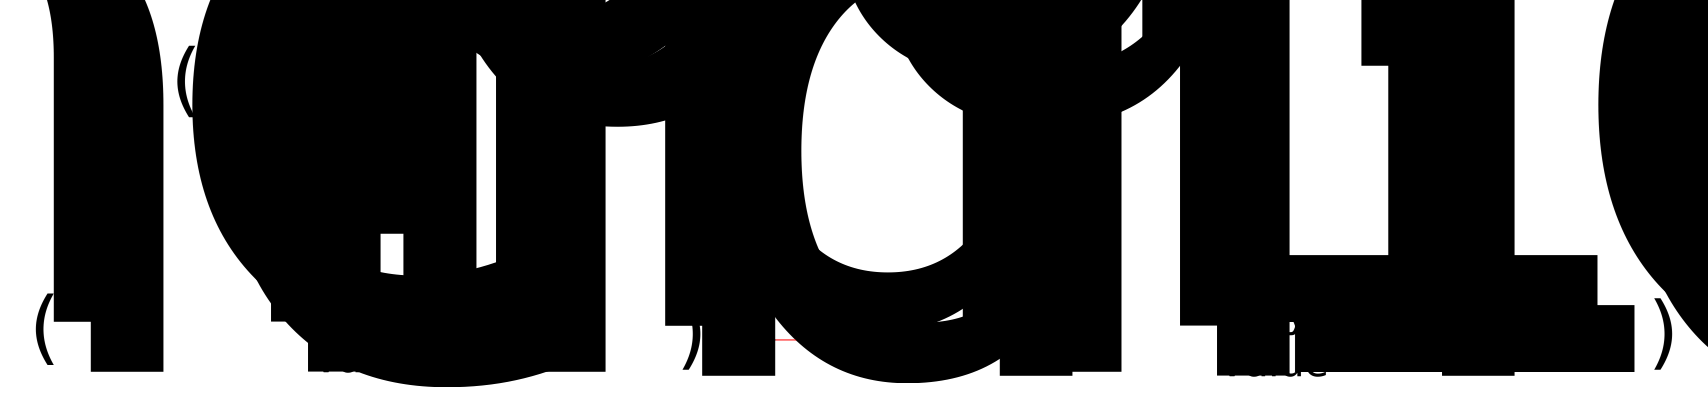
\includegraphics[width=\textwidth]{sidestep_explanation.pdf}
	\caption{
	\label{fig:sidestep}	
	When adding \textit{child2} as a child in direction \textcircled{b} (the black arrow) to \textit{parent} in the existing tree at a location that is already taken, the DHT server takes a \textit{side-step} in direction \textcircled{a} (the red arrow), keeping \textit{child2}'s position in direction \textcircled{b} correct. }
\end{figure}

When considering a key-space of two (or more) dimensions in this way, we have what might be named a \textbf{shuffled-branch tree}: The nodes of the tree are certain to be in their intended level,but the actual order of all child nodes branching downwards from a certain node might differ between DHT servers.\\

Because the order of nodes might differ between DHT servers, when inserting a child node to the shuffled-branch tree, it is possible that it is added as a child to the `wrong` parent node. Therefore, we cannot assume that the child $\leftrightarrow$ parent relationship is always correct. Thus, a shuffled-branch tree can be seen as a (possibly multidimensional) ordered list of unordered sets.\\

This might make it seem as if a shuffled-branch tree is not very useful, but that is not true. The property of \textit{discovery} on top of a distributed hash table, where access to finding new versions/variants of a certain $(key,value)$ pair can be limited to certain groups of persons in a multitude of ways (which can be chosen based on application requirements) is very powerful. 



% Fault-tolerance?
When a value is removed from the DHT because of a technical failure, and thus there is an empty spot in the list of consecutive iterative hashes, an naive version of the algorithm that finds all values in the shuffled-branch tree will stop at this position. To improve Fault Tolerance, we could specify a number of \textit{minimal consecutive hashes that have to be null}. Then, these empty spots are skipped.

This value probably does not need to be very large, as it lies in the nature of a Distributed Hash Table to make the risk of such a failure as small as possible. Also, when new elements are inserted in the given direction, the empty spots will be filled by these new elements.


\section{The Distributed Hash Tree}
Although the shuffled-branch tree provides \textit{discovery} and a good degree of \textit{fault tolerance}, the other wanted features still have to be implemented.\\


To implement these features on top of the shuffled-branch tree, we add new fields inside of the $value$ of the $(key,value)$ pair\footnote{These fields inside of the value might be stored in the DHT using any serialization scheme, such as JSON or BEncoding.}:


\begin{description}
	\item[\texttt{content}] The actual data we want to save. This data might be encrypted using any possibly asynchronous encryption scheme, to ensure \textbf{secrecy}.
	\item[\texttt{reference}] A reference to the \textbf{label}\footnote{in other words: the same value as contained in that node's label field.} of an earlier node, or \textit{null} in the case of the root node.
	\item[\texttt{label}] This label is computed by taking $hash(content \parallel reference)$\footnote{This one-way hashing function does not have to be the same as the one used for the shuffled-tree hashes, although it can be.}. By using the reference in the computation for the label as well, we create a chain of dependencies similar to what happens in a Merkle Tree\footnote{%TODO: Reference to Merkle Trees.
	Although in a merkle tree, parents contain hashes of their children, while in the Distributed-Hash Tree the children contain the hash of their parent.}. It is impossible to tamper with the data or the reference of any value in the chain to the root without invalidating that node and the nodes further down in the chain. This ensures \textbf{\texttt{immutability}} and \textbf{exact versioning}.
	\item[\texttt{signature}] This is a signature of of above fields $signature(content \parallel reference \parallel label)$, computed using a digital signature algorithm\footnote{Examples are the (Elliptic Curve) Digital Signing Algorithm, the Lamport Signature Algorithm, or the Rabin Signature Algorithm.}. Clients should only trust (and thus include in their representation of the Distributed Hash Table) nodes that have a valid and verified signature. This ensures \textbf{authorization}, as well as another layer of \textbf{immutability}.
\end{description}

As it is possible to travel in shuffled-branch direction \texttt{a)} by only knowing the current key, and this information is known to untrusted parties such as the DHT server's owners, it is possible for these parties to insert extra (possibly malicious) values in the \texttt{a)} direction. But, as they are unable to create a proper signature, these values will be rejected by the users of that specific Distributed Hash Tree. This also means that in the unlikely event that the Distributed Hash Trees used by two different groups start sharing part of each other's key-space, the groups will simply reject each other's nodes as invalid.

Instead of encrypting the data, it is also possible to encrypt the whole set of fields inside the DHT's $value$. The advantage is that the relationships between nodes might be harder to see for third parties\footnote{Although this is already hard because one can only travel one-way inside the shuffled-hash tree, so the third parties would need earlier hashes to see more of the referenced nodes.}. The disadvantage is that this means that the user needs to decrypt \textbf{all} nodes before knowing which one was referred to.

\section{Conclusion}


\end{document}

% Rewrite/Remove this paragraph?
One way to ensure this uniqueness is by using a one-way hashing function\footnote{examples of one-way hashing functions here} on the value. The advantage is that it becomes (nearly\footnote{pidgeonhole principle}) impossible for two differing values to have a key-collision. The drawback of this is that, when knowing only the key, it is impossible to find any other versions, as it is impossible to link key hashes this way.